\begin{center}
\section{Project Management}
\label{waterfall}
\end{center}

Before the official project start date, a feasibility study was conducted, including the creation of a simple prototype over the 2024 summer break to validate the algorithm. In doing so, it highlighted opportunities for future work and areas of improvement. The work conducted could not be transferred to the main project, as an entire redesign of the system was necessary with the addition of TSP\_Data and the project's planned features.

At the start of the project, a proposed timeline defining the development of major features was produced(Figure\ref{fig:timeline}). Key milestones were identified that needed to be reached before moving on, as each system was built on top of the other. This led to the natural conclusion of using the waterfall project management model\cite{thesing2021agile}, requiring each step to design, implement, and test the current feature. This process ensured that backtracking or refactoring was not needed as the trust in existing code for future development was guaranteed.

\begin{figure}[H]
    \centering
    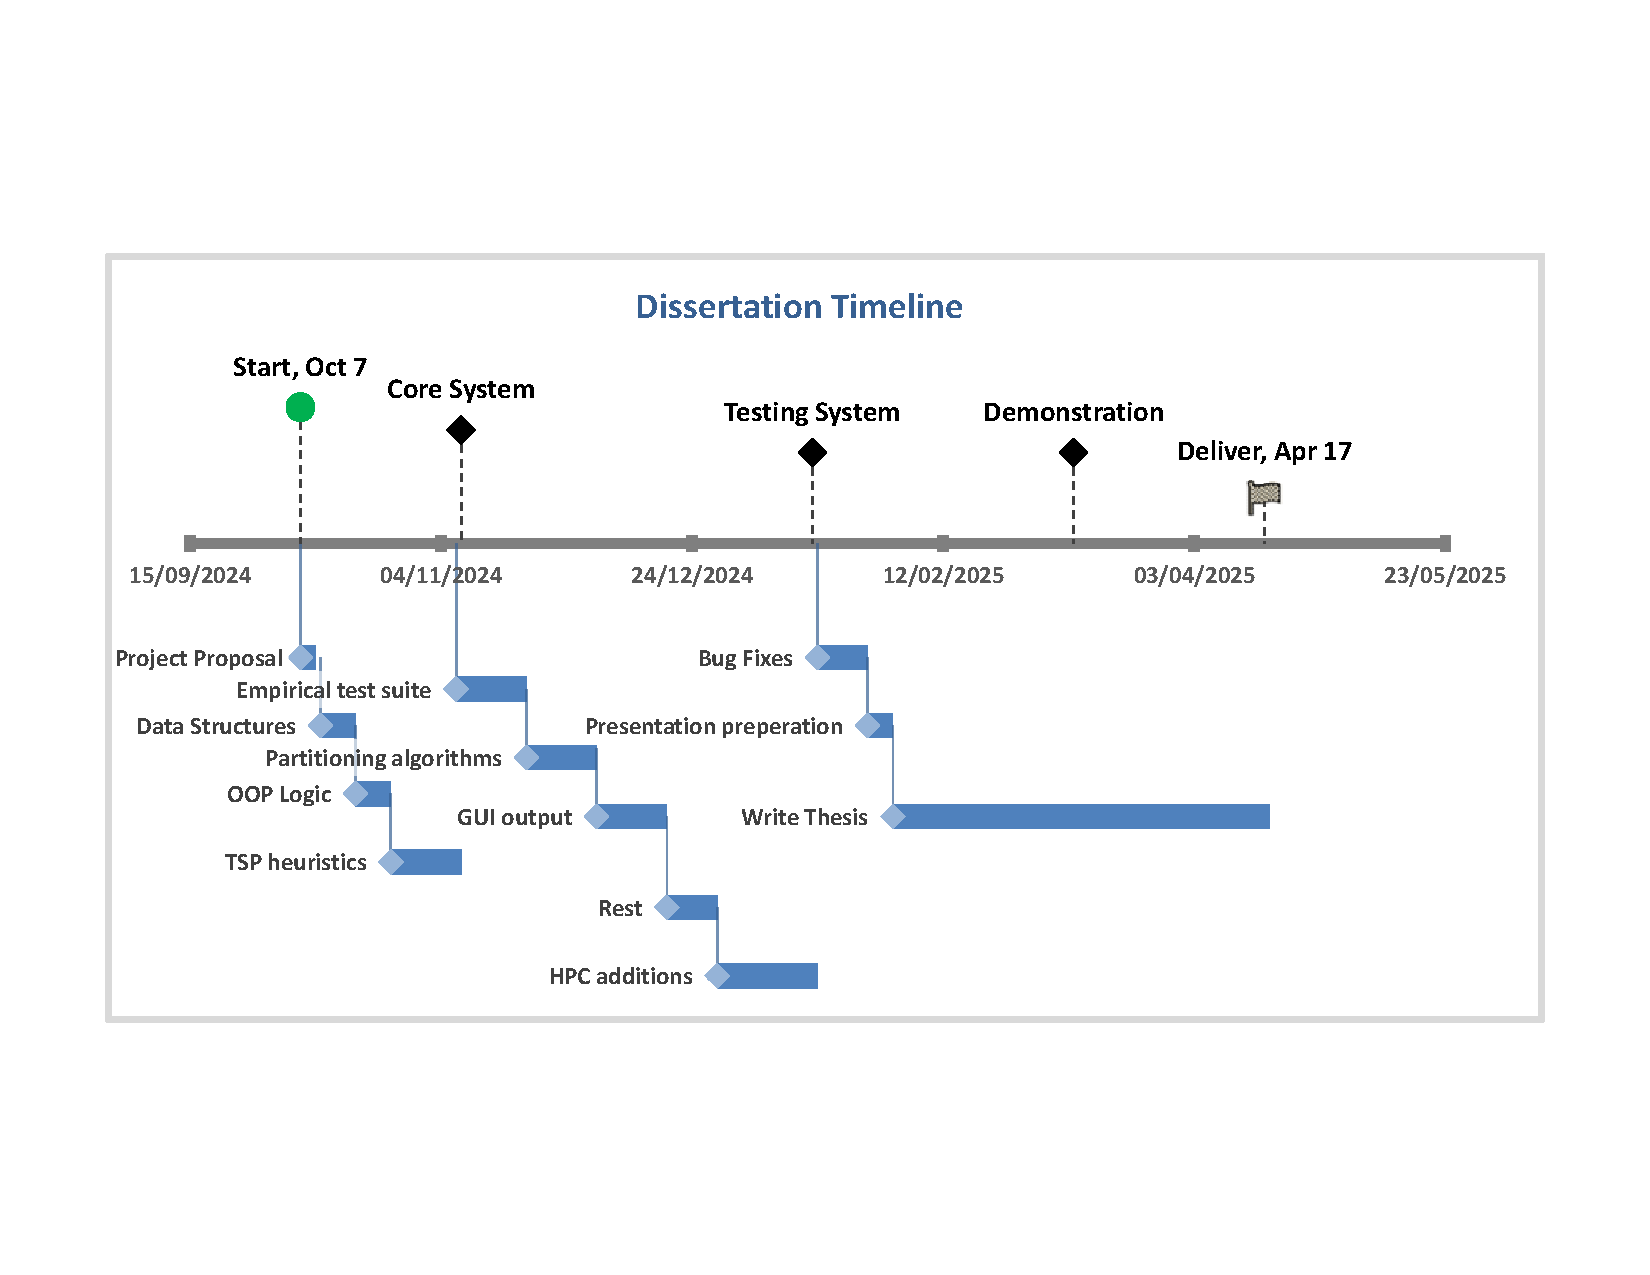
\includegraphics[width=0.9\textwidth]{sections/image/timeline.pdf}
    \caption{Project Timeline}
    \label{fig:timeline}
\end{figure}

The major milestones split the project between the core system(TSP Library) and application-specific development. Both of the major milestones had minor milestones that structured the development process of each system(Figure\ref{fig:timeline}). Similar to many projects, the project overran due to ambitious goals, leading to the high-performance computing feature being removed from the project scope in order to meet the final delivery date. Nonetheless, the quality of work and development efficiency achieved throughout the project were the highest delivered.